\subsection{Setzeinheit} \label{sec:Inbetriebnahme_Setzeinheit}
\textit{(pro)} Ähnlich wie ION Motion bietet auch Trinamic eine eigene PC Software für die Ansteuerung ihrer Motorencontroller an. Trinamic nennt das Tool dabei TMCL-IDE. Die TMCL-IDE wurde für eine ganze Familie von Motorencontroller entwickelt. Diese Software ist sehr umfangreich und bietet Tools zur Identifikation des verwendeten Motors sowie dessen Hall Sensoren, zur Bestimmung von Regelparameter, Programmierung von Bewegungsabläufen und vielem mehr. In Abb. \ref{fig:TMCL-IDE} ist ein Auszug der Software zu sehen.

\begin{figure}[H]
	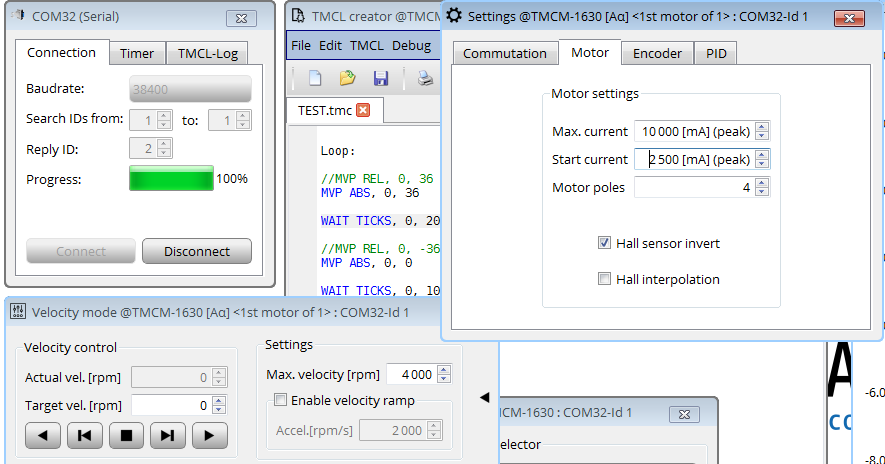
\includegraphics[width=0.7\textwidth]{Illustrationen/7-Inbetriebnahme_und_Kalibration/TMCL_IDE.png}
	\caption{Trinamic TMCL IDE}
	\label{fig:TMCL-IDE}
\end{figure}

Im Umfang dieses Projekts wurde mit Hilfe dieser Software der Bewegungsablauf der Setzeinheit eingestellt und durch verändern der Regelparameter zu einer flüssigen Bewegung optimiert. Für eine optimale Auslastung der Hardware hätte in diesem Teil der Inbetriebnahme noch mehr Zeit investiert werden sollen. Der getestete Bewegungsablauf wurde anschliessend auf die Software des FRDM-Boards adaptiert. Weiter wurde auch die Initialisierungphase erfolgreich getestet, bei der die Setzeinheit an den oberen Anschlag fährt.

\subsection{Stechdorn}
\begin{figure}[H]
	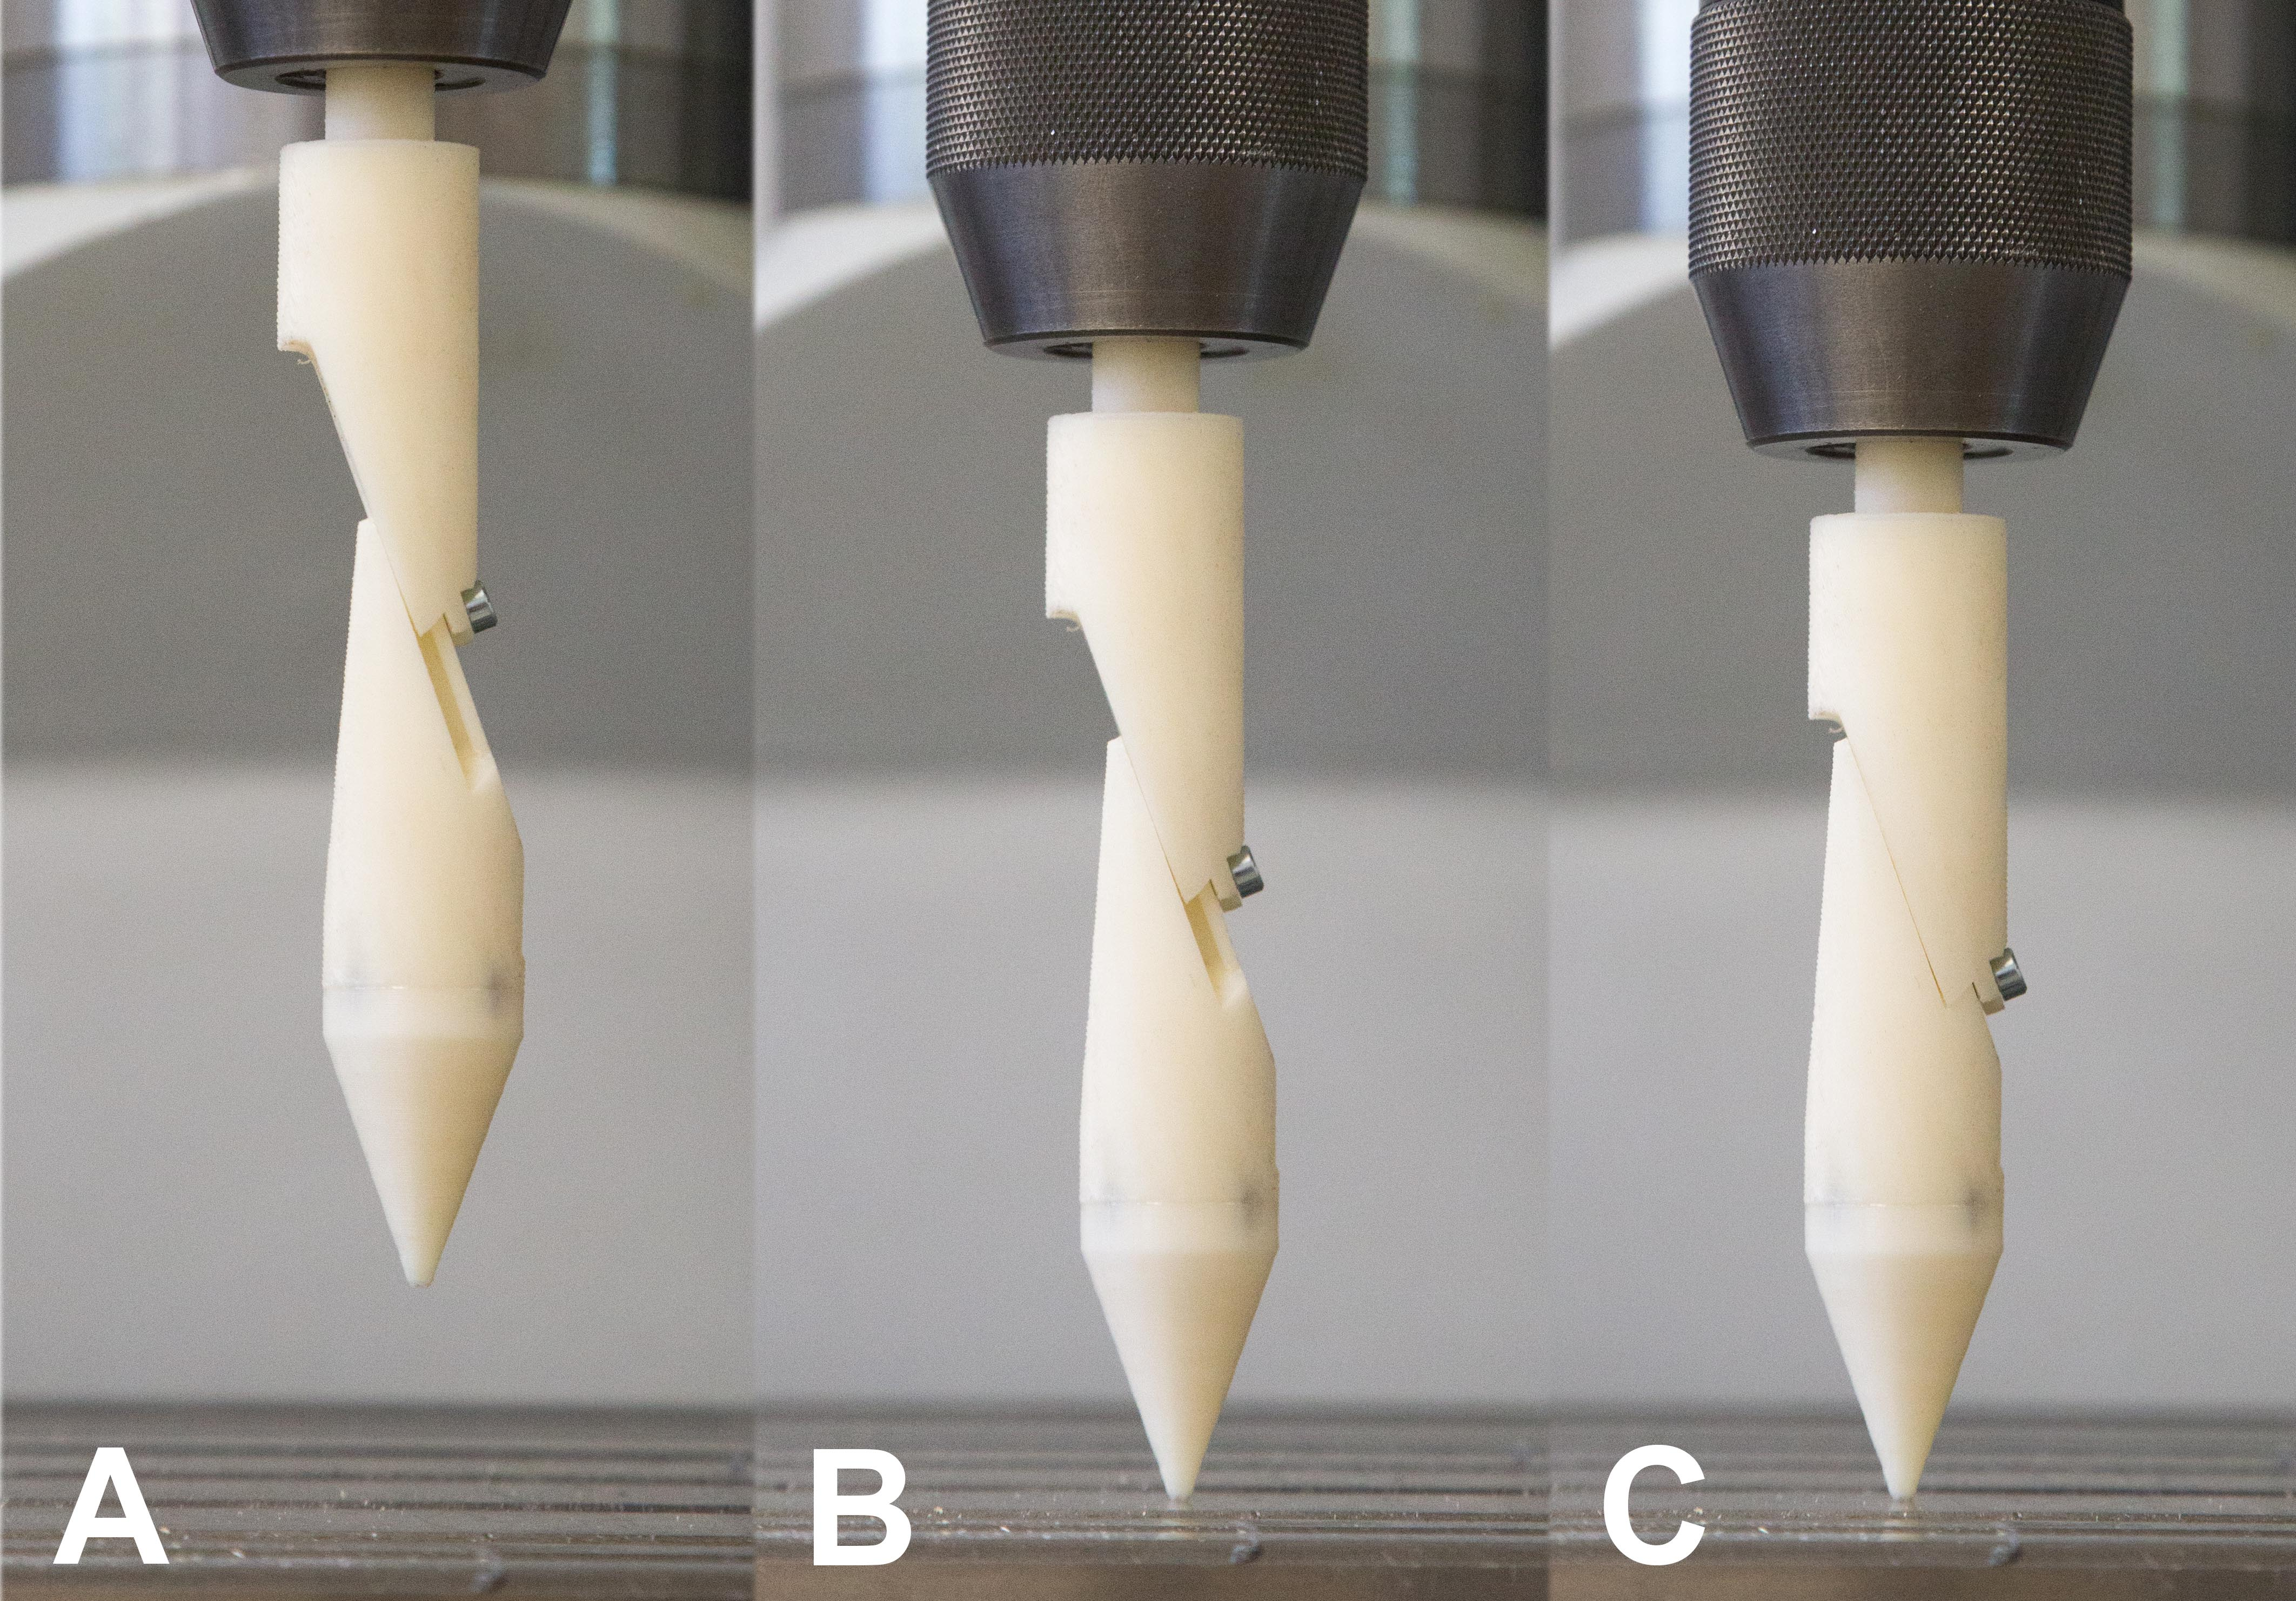
\includegraphics[width=0.7\textwidth]{Illustrationen/7-Inbetriebnahme_und_Kalibration/inbet_stechdorn.jpg}
	\caption{Schliessvorgang des Stechdorns}
	\label{fig:inbet_stechdorn}
\end{figure}